\section{Guardian Characteristics}
\begin{frame}
 \frametitle{Hardware implementation}

 \begin{textblock*}{5cm}(7.5cm,5.5cm)
  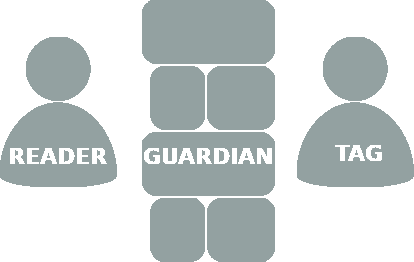
\includegraphics[scale=0.15]{Guardian}
 \end{textblock*}

 \begin{textblock*}{5cm}(1.2cm,2.2cm)
  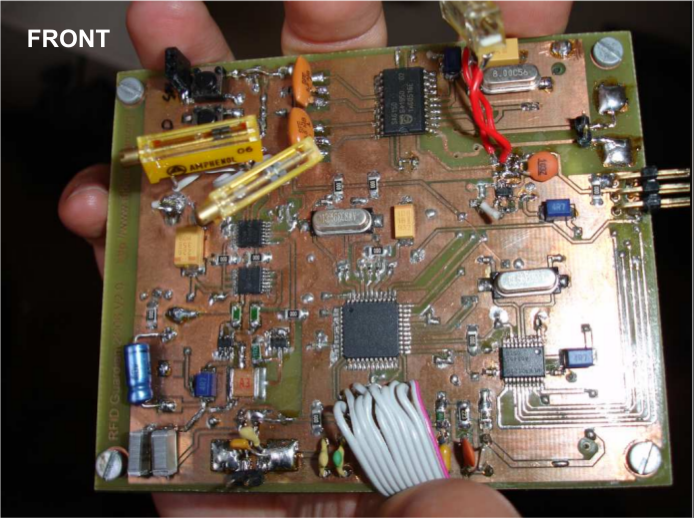
\includegraphics[scale=0.25]{FrontGuardian}
 \end{textblock*}

 \begin{textblock*}{5cm}(6.5cm,3cm)
  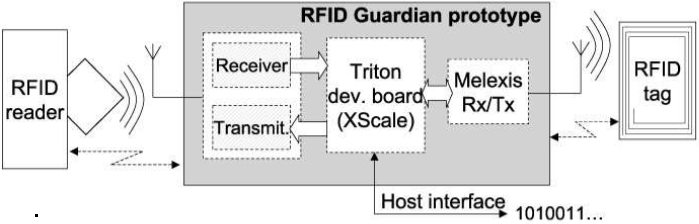
\includegraphics[scale=0.3]{GuardianScheme}
 \end{textblock*}

 \begin{textblock*}{5cm}(1cm,6.5cm)
  \begin{itemize}
   \item RFID Guardian act like a wall between the reader and the tag
  \end{itemize}
 \end{textblock*}

\end{frame}

\begin{frame}
 \frametitle{Software implementation}

 \begin{itemize}
  \item<1-> Real time OS (e-Cos real time operating system)
  \item<2-> In this OS each functionality is a task:
  \begin{itemize}
   \item Timer
   \item User Input
   \item Tag
   \item Reader
  \end{itemize}

 \end{itemize}


\end{frame}
